\documentclass[a4paper]{scrartcl}
\usepackage[cm]{fullpage}
\usepackage{amsmath, amssymb}
\usepackage{siunitx}
\usepackage{graphicx, caption, subcaption}

\begin{document}

\title{PHYS1241: Faraday's Law}
\author{ \\ \\ }
\date{2015-09-10}
\maketitle

\section{Abstract}
The validity of Faraday's law of induction was found to hold true by using it to calculate the flux through multiple types of solenoids when an identical magnet is dropped through them.

\section{Introduction}
Induction is critical to our electricity infrastructure, driving the generators that power it, but we have not experienced it for ourselves in the lab yet. This experiment serves to do that, as well as confirm that Faraday's law of induction holds true in the presence of a changing magnetic field.

\section{Materials and Methods}
Please refer to page 96 in the PHYS1241 laboratory manual for the materials used.

The tube was placed through the solenoid's axis vertically to ensure the magnet would pass smoothly through the solenoid. The magnet was then released from the top of the tube and the induced EMF with respect to time was recorded. This was done for solenoids of 200, 400 and 800 loops.

If Faraday's law, that is \(V = -N \frac{\mathrm{d}\Phi_B}{\mathrm{d}t}\), were to hold, then integrating through and rearranging would produce the following equation:
\[\Delta\Phi_B = \frac{-\int_0^t V \,\mathrm{d}t}{N}\]

Since the magnet used would be the same between each attempt, the maxima of \(\Delta\Phi_B\) should remain the same regardless of the number of loops in the solenoid and the speed the magnet passes through it. Thus, comparing the maxima between multiple attempts and seeing if they coincide would test for Faraday's law.

Error was calculated by considering the end value of our \(\Delta\Phi_B\). In a perfectly measured result, this should equal zero, but due to errors in our voltmeter and numerical integration, it will unlikely be equal to zero in practice. Therefore, this value can be considered the error in \(\Delta\Phi_B\).

Originally, we planned to compared the plot of \(-\int_0^t V \,\mathrm{d}t\) to \(N B A\) by measuring both the induced EMF, and the magnetic field at the solenoid's opening, respectively. However, the magnetic field probe was unable to read the field strength of the magnets we used and clipped the value at a value much lower than the real value, so this method was discarded.

\section{Results}
\begin{table}
    \centering
    \begin{tabular}{c | c}
        Loops & Max \(\Delta\Phi_B\) (\si{\micro\weber}) \\
        \hline
        200 & \SI{7.6 \pm 1.2}{} \\
        200 & \SI{7.4 \pm 2.1}{} \\
        200 & \SI{7.7 \pm 0.4}{} \\
        400 & \SI{8.1 \pm 0.1}{} \\
        400 & \SI{7.9 \pm 0.2}{} \\
        400 & \SI{7.5 \pm 1.1}{} \\
        800 & \SI{8.2 \pm 0.3}{} \\
        800 & \SI{8.2 \pm 1.7}{} \\
        800 & \SI{8.2 \pm 0.3}{} \\
        \hline
    \end{tabular}
    \caption{Maximum \(\Delta\Phi_B\) observed}
    \label{tab:max_phi}
\end{table}

Figures \ref{fig:200_1} to \ref{fig:800_3} shows the raw data recorded and analysed, with the maximum \(\Delta\Phi_B\) values in Table \ref{tab:max_phi}.

\section{Discussion}
From the values presented in Table \ref{tab:max_phi}, it can be clearly seen that a flux of approximately \SI{8}{\micro\weber} fits within error of all the values. The graphs of the EMF and flux against time are also in the expected general shape.

From these results, it can be seen that Faraday's law holds true.

However, since we are only considering a single point of the flux, this experiment can be greatly improved by using a magnetic field probe that is strong enough to measure the full field strength of the magnet and using the original discarded method that considers the entire flux graph.

Alternatively, this very same experiment could be repeated with a more powerful magnet and a more sensitive voltmeter to increase the resolution accuracy in the measured EMF to reduce the variation in the results, especially evident in the graphs for 200 loops.

\begin{figure}[p]
    \centering
    \begin{subfigure}[b]{0.45\textwidth}
        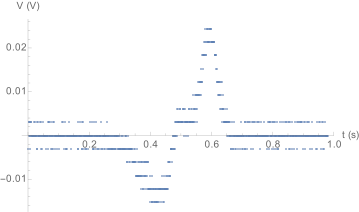
\includegraphics[width = \textwidth]{200_1_voltage.png}
        \caption{Measured EMF}
    \end{subfigure}
    ~
    \begin{subfigure}[b]{0.45\textwidth}
        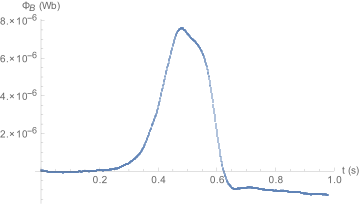
\includegraphics[width = \textwidth]{200_1_flux.png}
        \caption{Calculated Flux}
    \end{subfigure}
    \caption{200 Loops - Attempt 1}
    \label{fig:200_1}
\end{figure}
\begin{figure}[p]
    \centering
    \begin{subfigure}[b]{0.45\textwidth}
        \includegraphics[width = \textwidth]{200_2_voltage.png}
        \caption{Measured EMF}
    \end{subfigure}
    ~
    \begin{subfigure}[b]{0.45\textwidth}
        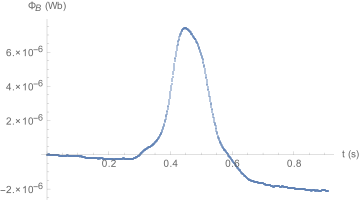
\includegraphics[width = \textwidth]{200_2_flux.png}
        \caption{Calculated Flux}
    \end{subfigure}
    \caption{200 Loops - Attempt 2}
    \label{fig:200_2}
\end{figure}
\begin{figure}[p]
    \centering
    \begin{subfigure}[b]{0.45\textwidth}
        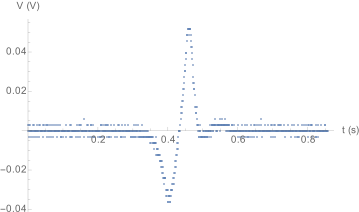
\includegraphics[width = \textwidth]{200_3_voltage.png}
        \caption{Measured EMF}
    \end{subfigure}
    ~
    \begin{subfigure}[b]{0.45\textwidth}
        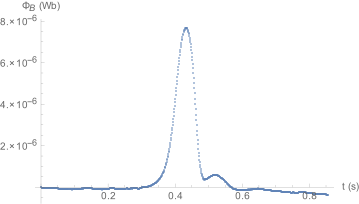
\includegraphics[width = \textwidth]{200_3_flux.png}
        \caption{Calculated Flux}
    \end{subfigure}
    \caption{200 Loops - Attempt 3}
    \label{fig:200_3}
\end{figure}

\begin{figure}[p]
    \centering
    \begin{subfigure}[b]{0.45\textwidth}
        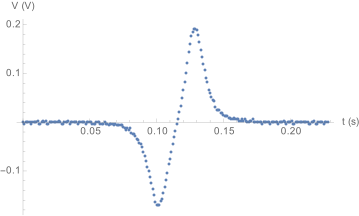
\includegraphics[width = \textwidth]{400_1_voltage.png}
        \caption{Measured EMF}
    \end{subfigure}
    ~
    \begin{subfigure}[b]{0.45\textwidth}
        \includegraphics[width = \textwidth]{400_1_flux.png}
        \caption{Calculated Flux}
    \end{subfigure}
    \caption{400 Loops - Attempt 1}
    \label{fig:400_1}
\end{figure}
\begin{figure}[p]
    \centering
    \begin{subfigure}[b]{0.45\textwidth}
        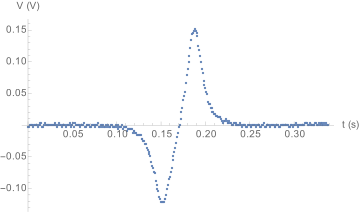
\includegraphics[width = \textwidth]{400_2_voltage.png}
        \caption{Measured EMF}
    \end{subfigure}
    ~
    \begin{subfigure}[b]{0.45\textwidth}
        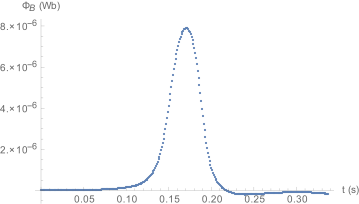
\includegraphics[width = \textwidth]{400_2_flux.png}
        \caption{Calculated Flux}
    \end{subfigure}
    \caption{400 Loops - Attempt 2}
    \label{fig:400_2}
\end{figure}
\begin{figure}[p]
    \centering
    \begin{subfigure}[b]{0.45\textwidth}
        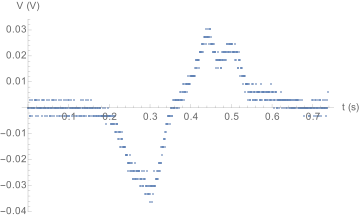
\includegraphics[width = \textwidth]{400_3_voltage.png}
        \caption{Measured EMF}
    \end{subfigure}
    ~
    \begin{subfigure}[b]{0.45\textwidth}
        \includegraphics[width = \textwidth]{400_3_flux.png}
        \caption{Calculated Flux}
    \end{subfigure}
    \caption{400 Loops - Attempt 3}
    \label{fig:400_3}
\end{figure}


\begin{figure}[p]
    \centering
    \begin{subfigure}[b]{0.45\textwidth}
        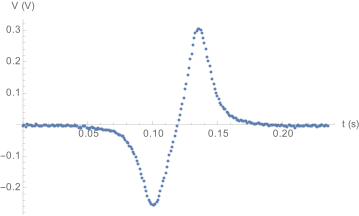
\includegraphics[width = \textwidth]{800_1_voltage.png}
        \caption{Measured EMF}
    \end{subfigure}
    ~
    \begin{subfigure}[b]{0.45\textwidth}
        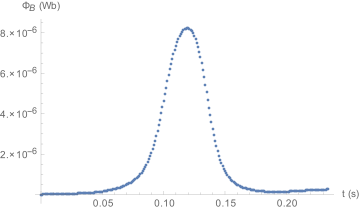
\includegraphics[width = \textwidth]{800_1_flux.png}
        \caption{Calculated Flux}
    \end{subfigure}
    \caption{800 Loops - Attempt 1}
    \label{fig:800_1}
\end{figure}
\begin{figure}[p]
    \centering
    \begin{subfigure}[b]{0.45\textwidth}
        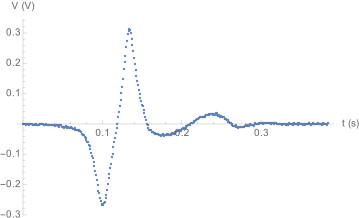
\includegraphics[width = \textwidth]{800_2_voltage.png}
        \caption{Measured EMF}
    \end{subfigure}
    ~
    \begin{subfigure}[b]{0.45\textwidth}
        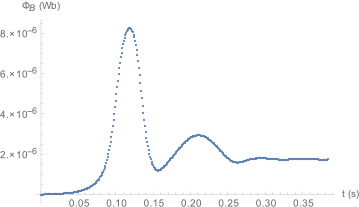
\includegraphics[width = \textwidth]{800_2_flux.png}
        \caption{Calculated Flux}
    \end{subfigure}
    \caption{800 Loops - Attempt 2}
    \label{fig:800_2}
\end{figure}
\begin{figure}[p]
    \centering
    \begin{subfigure}[b]{0.45\textwidth}
        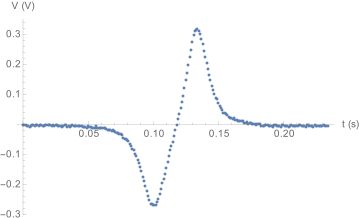
\includegraphics[width = \textwidth]{800_3_voltage.png}
        \caption{Measured EMF}
    \end{subfigure}
    ~
    \begin{subfigure}[b]{0.45\textwidth}
        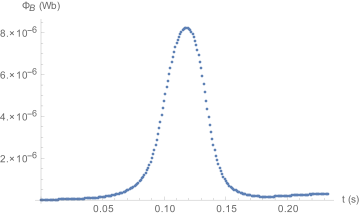
\includegraphics[width = \textwidth]{800_3_flux.png}
        \caption{Calculated Flux}
    \end{subfigure}
    \caption{800 Loops - Attempt 3}
    \label{fig:800_3}
\end{figure}

\end{document}
